



%%%%%%%%%%%%%%%%%%%%%%%%%%%%%%%%%%%%%%%%%
% Beamer Presentation
% LaTeX Template
% Version 1.0 (10/11/12)
%
% This template has been downloaded from:
% http://www.LaTeXTemplates.com
%
% License:
% CC BY-NC-SA 3.0 (http://creativecommons.org/licenses/by-nc-sa/3.0/)
%
%%%%%%%%%%%%%%%%%%%%%%%%%%%%%%%%%%%%%%%%%

%----------------------------------------------------------------------------------------
%	PACKAGES AND THEMES
%----------------------------------------------------------------------------------------

\documentclass[aspectratio=169]{beamer}

\mode<presentation> {


% The Beamer class comes with a number of default slide themes
% which change the colors and layouts of slides. Below this is a list
% of all the themes, uncomment each in turn to see what they look like.

%\usetheme{default}
%\usetheme{AnnArbor}
%\usetheme{Antibes}
%\usetheme{Bergen}
%\usetheme{Berkeley}
%\usetheme{Berlin}
%\usetheme{Boadilla}
%\usetheme{CambridgeUS}
%\usetheme{Copenhagen}
%\usetheme{Darmstadt}
%\usetheme{Dresden}
%\usetheme{Frankfurt}
%\usetheme{Goettingen}
%\usetheme{Hannover}
%\usetheme{Ilmenau}
%\usetheme{JuanLesPins}
%\usetheme{Luebeck}
\usetheme{Madrid}
%\usetheme{Malmoe}
%\usetheme{Marburg}
%\usetheme{Montpellier}
%\usetheme{PaloAlto}
%\usetheme{Pittsburgh}
%\usetheme{Rochester}
%\usetheme{Singapore}
%\usetheme{Szeged}
%\usetheme{Warsaw}

% As well as themes, the Beamer class has a number of color themes
% for any slide theme. Uncomment each of these in turn to see how it
% changes the colors of your current slide theme.

%\usecolortheme{albatross}
%\usecolortheme{beaver}
%\usecolortheme{beetle}
%\usecolortheme{crane}
%\usecolortheme{dolphin}
%\usecolortheme{dove}
%\usecolortheme{fly}
%\usecolortheme{lily}
%\usecolortheme{orchid}
%\usecolortheme{rose}
%\usecolortheme{seagull}
%\usecolortheme{seahorse}
%\usecolortheme{whale}
%\usecolortheme{wolverine}

%\setbeamertemplate{footline} % To remove the footer line in all slides uncomment this line
%\setbeamertemplate{footline}[page number] % To replace the footer line in all slides with a simple slide count uncomment this line
\usepackage{amsmath}
\usepackage{selinput}      % Halbautomatische Auswahl der Eingabecodierung
\SelectInputMappings{      % mit Hilfe ausgewählter Glyphen
  adieresis={ä},	   % siehe: http://partners.adobe.com/public/developer/en/opentype/glyphlist.txt
  germandbls={ß},
  Euro={€}
}

\definecolor{UOSred}{rgb}{0.6745098039215686, 0.02352941176470588, 0.2039215686274510} % UBC Blue (primary)
\definecolor{UOSgrey}{rgb}{0.8117647058823529, 0.8117647058823529, 0.8117647058823529} % UBC Grey (secondary)

\setbeamercolor{palette primary}{bg=UOSred,fg=white}
\setbeamercolor{palette secondary}{bg=UOSred,fg=white}
\setbeamercolor{palette tertiary}{bg=UOSred,fg=white}
\setbeamercolor{palette quaternary}{bg=UOSred,fg=white}
\setbeamercolor{structure}{fg=UOSred} % itemize, enumerate, etc
\setbeamercolor{section in toc}{fg=UOSred} % TOC sections

%gets rid of bottom navigation bars
\setbeamertemplate{footline}[frame number]{}

%gets rid of bottom navigation symbols
\setbeamertemplate{navigation symbols}{}

\addtobeamertemplate{footline}{%
  \leavevmode%
  \hbox{%
  \begin{beamercolorbox}[wd=\paperwidth,ht=2.25ex,dp=1ex,center]{author in head/foot}%
     \insertsectionnavigationhorizontal{\paperwidth}{}{}
  \end{beamercolorbox}}%

}

% Override palette coloring with secondary
\setbeamercolor{subsection in head/foot}{bg=UOSgrey,fg=white}

%\setbeamertemplate{navigation symbols}{} % To remove the navigation symbols from the bottom of all slides uncomment this line
}
\usepackage{hyperref}
\usepackage{graphicx} % Allows including images
\usepackage{grffile}
\usepackage{booktabs} % Allows the use of \toprule, \midrule and \bottomrule in tables
\graphicspath{{images/}}
%----------------------------------------------------------------------------------------
%	TITLE PAGE
%----------------------------------------------------------------------------------------

\title[Aufgabe 1.1]{Aufgabe 3.1} % The short title appears at the bottom of every slide, the full title is only on the title page

\author{T. Adam, M. ben Ahmed} % Your name
\institute[UOS] % Your institution as it will appear on the bottom of every slide, may be shorthand to save space
{

Universität Osnabrück \\ % Your institution for the title page

\medskip
\textit{Æ} % Your email address


}
\date{\today} % Date, can be changed to a custom date

\begin{document}

\begin{frame}
\titlepage % Print the title page as the first slide
\end{frame}


%----------------------------------------------------------------------------------------
%	PRESENTATION SLIDES
%----------------------------------------------------------------------------------------


%------------------------------------------------



\begin{frame}
	\frametitle{Aufgabe 3.1 - Übersicht}
	\begin{columns}[c] % The "c" option specifies centered vertical alignment while the "t" option is used for top vertical alignment
		
		\column{.40\textwidth} % Left column and width
		\textbf{Testen von Suchbaum Layouts}
		\begin{itemize}
			\item zufällig
			\item sortiert
			\item level-weise
			\item van Emde Boas
		\end{itemize}

		\column{.35\textwidth} % Right column and width
		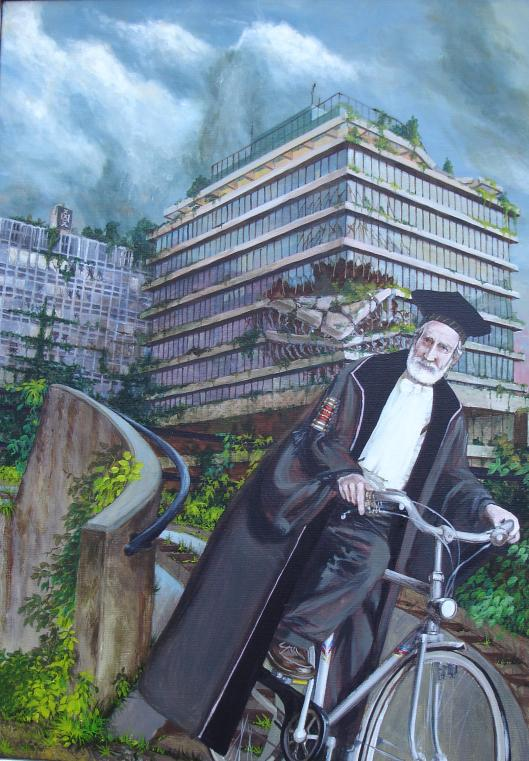
\includegraphics[scale=.2]{portretPeter.jpg}
		\tiny \texttt{\url{https://staff.fnwi.uva.nl/p.vanemdeboas/}}
		
		
	\end{columns}
	\end{frame}
	
%------------------------------------------------

\begin{frame}
	\frametitle{Aufgabe 3.1 - (Perfekt) balancierter binärer Suchbaum}
	
	\textbf{Baumstruktur}
	\begin{itemize}
		\item Perfekt balancierter binärer Suchbaum
		\item linker Kindknoten $<$ Elternknoten $<$ rechter Kindknoten
		\item $n$ Level
		\item $2^{n}-1$ Schlüssel
		\item Integerarray speichert die Schlüssel
	\end{itemize}

	\end{frame}
%------------------------------------------------

\begin{frame}
	\frametitle{Aufgabe 3.1 - Zufällig}
	
	\begin{center}
		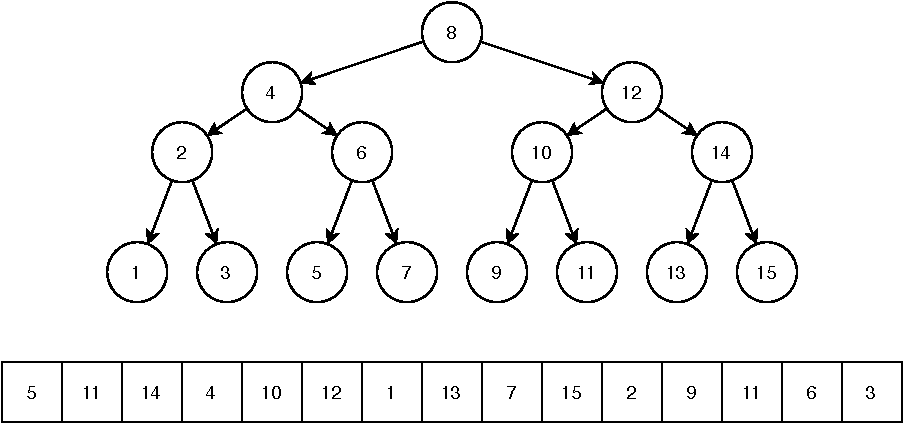
\includegraphics[scale=.8]{random_layout.pdf}\\
		\centering \texttt{find(key)}: iteriere über array
	\end{center}

	\end{frame}
%------------------------------------------------

\begin{frame}
	\frametitle{Aufgabe 3.1 - Aufsteigend sortiert}
	
	
	\begin{center}
		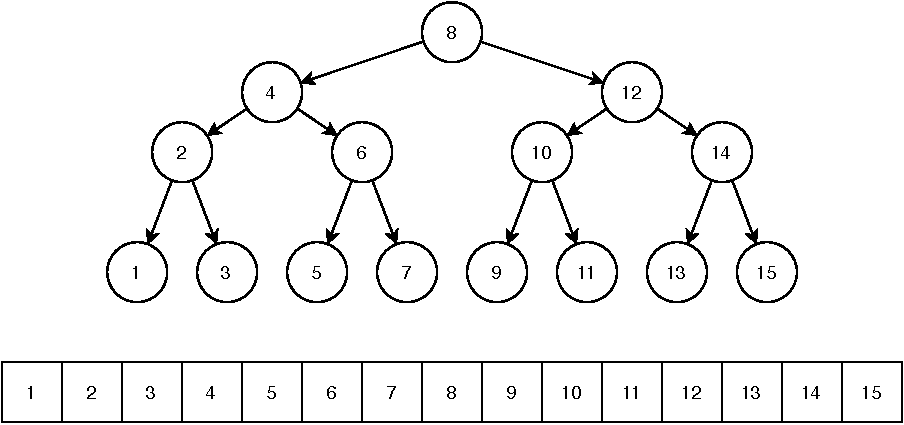
\includegraphics[scale=.8]{sorted_layout.pdf}\\
		\centering \texttt{find(key)}: binäre Suche	
	\end{center}
	\end{frame}
%------------------------------------------------


\begin{frame}
	\frametitle{Aufgabe 3.1 - Levelweise sortiert}
	
	
	\begin{center}
		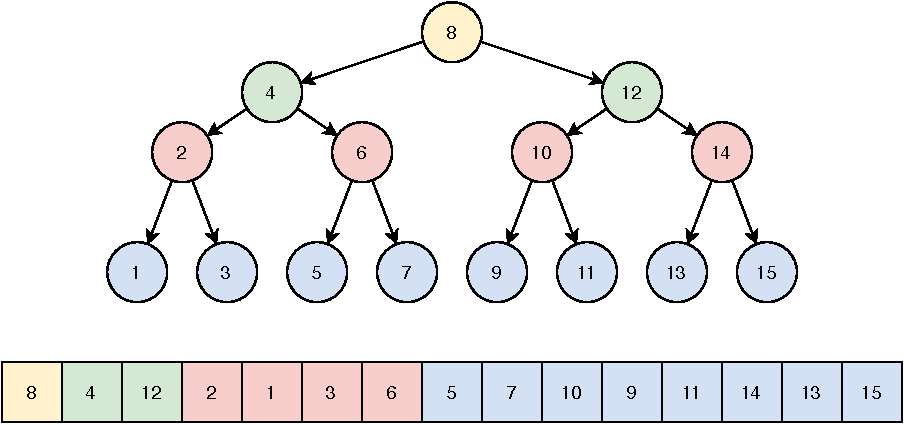
\includegraphics[scale=.8]{level_layout.pdf}\\
		\centering \texttt{find(key)}: $links(i) = 2i$, $rechts(i) = 2i+1$	
	\end{center}
	\end{frame}
%------------------------------------------------


\begin{frame}
	\frametitle{Aufgabe 3.1 - van Emde Boas Layout}
	
	
	\begin{center}
		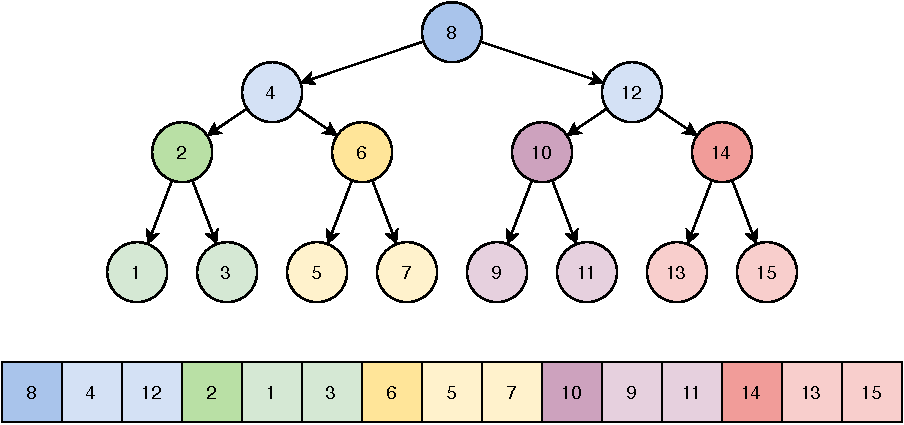
\includegraphics[scale=.8]{veb_layout.pdf}\\
		\centering \texttt{find(key)}: ???	
	\end{center}
	\end{frame}
%------------------------------------------------
\begin{frame}
	\frametitle{Aufgabe 3.1 - Berechnung der Indizes im VEB Layout}
	
	\textbf{Van Emde Boas Layout}
	\begin{itemize}
		\item wir betrachten zwei mögliche Implementationen
		\item es ist kein Konstantzeitalgorithmus für Indizeberechnung bekannt
		\item Konvertieren von \texttt{bfs}-Index zu VEB-Index in $\mathcal{O}(\log h)$
		\item alternative Implementation durch Zeiger auf Kindknoten
	\end{itemize}

	\end{frame}
%------------------------------------------------

\begin{frame}
\frametitle{Aufgabe 3.1 - Testmaschinen}
\begin{columns}[c] % The "c" option specifies centered vertical alignment while the "t" option is used for top vertical alignment
	
	\column{.30\textwidth} % Left column and width
	\textbf{Intel Core i5-3570K}
	\begin{itemize}
		\item 4c/4t
		\item 3,4 - 3,8 GHz
		\item 6 MB L3
		\item 8 GB (1600 MHz)
		\item Linux (Kubuntu 18.04)
		
	\end{itemize}
	
	\column{.30\textwidth} % Right column and width
	\textbf{Intel Core i7-3770K}
	\begin{itemize}
		\item 4c/8t
		\item 3,5 - 3,9 GHz
		\item 8 MB L3
		\item 16 GB (1600 MHz)
		\item Linux (Kubuntu 18.04)
		
	\end{itemize}
	

	\column{.30\textwidth} % Right column and width
	\textbf{Intel Core i7-8565U}
	\begin{itemize}
		\item 4c/8t
		\item 1,8 - 4,6 GHz
		\item 8MB L3
		\item 16 GB (2400 MHz)
		\item Linux (Arch)
	\end{itemize}

\end{columns}
\end{frame}

%------------------------------------------------

\begin{frame}
	\frametitle{Aufgabe 3.1 - Auswertung}
	\begin{columns}[c] % The "c" option specifies centered vertical alignment while the "t" option is used for top vertical alignment
		
		\column{.35\textwidth} % Left column and width
		\textbf{Vergleich der Layouts}
		\column{.6\textwidth} % Right column and width
		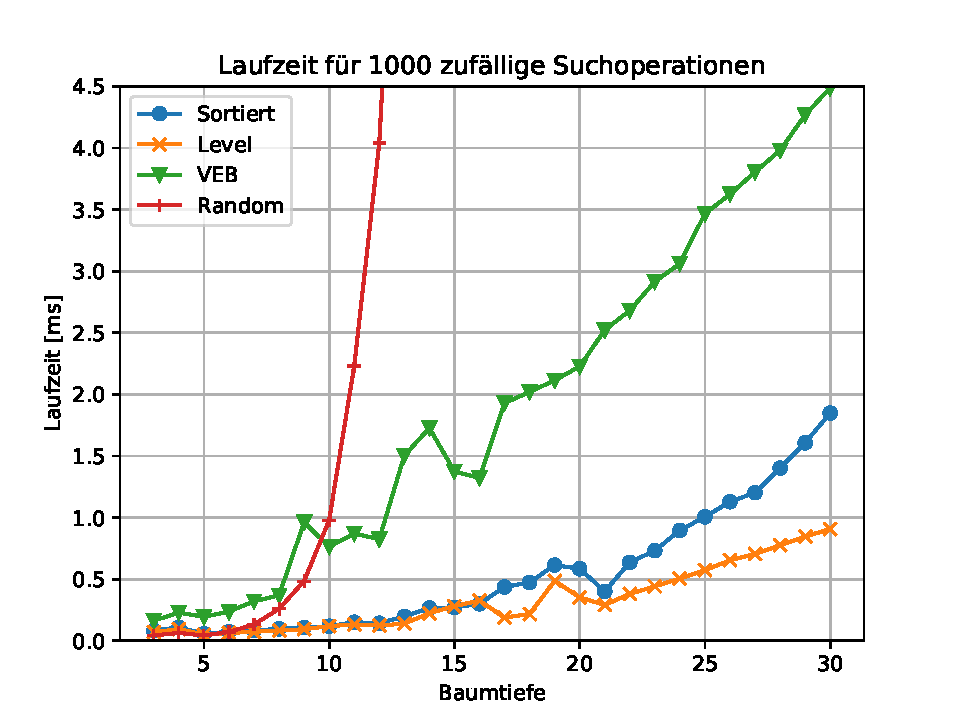
\includegraphics[scale=.6]{Figure_2.pdf}
		
		
	\end{columns}
	\end{frame}
	
%------------------------------------------------

\begin{frame}
	\frametitle{Aufgabe 3.1 - Auswertung}
	\begin{columns}[c] % The "c" option specifies centered vertical alignment while the "t" option is used for top vertical alignment
		
		\column{.35\textwidth} % Left column and width
		\textbf{Vergleich der Maschinen}
		\column{.6\textwidth} % Right column and width
		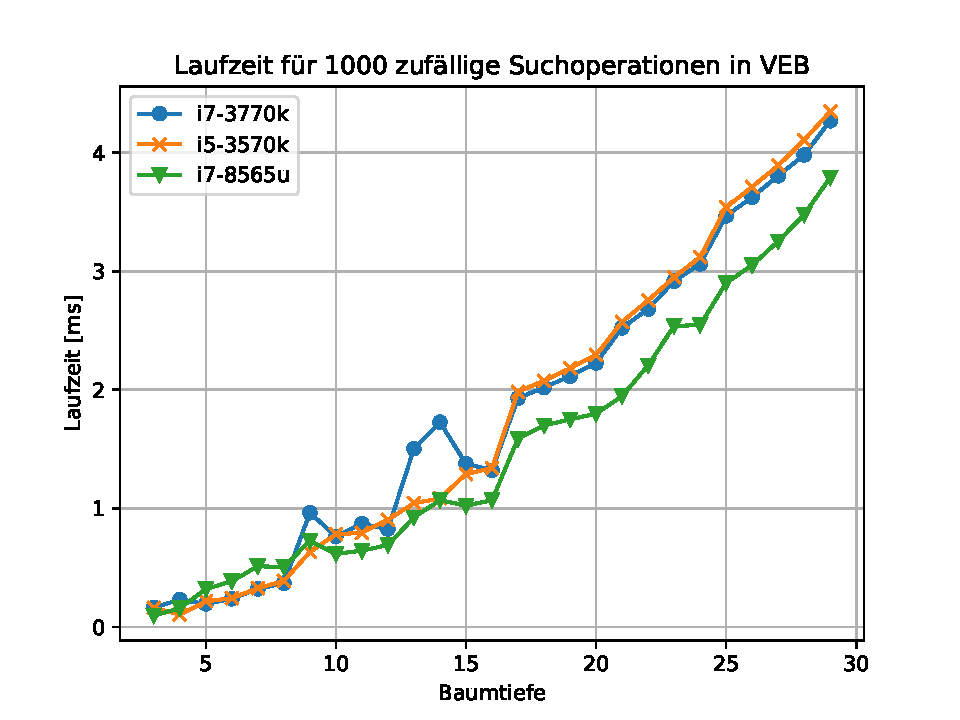
\includegraphics[scale=.6]{cpu_comp.pdf}
		
		
	\end{columns}
	\end{frame}
	
%------------------------------------------------


\begin{frame}
	\frametitle{Aufgabe 3.1 - Auswertung}
	\begin{columns}[c] % The "c" option specifies centered vertical alignment while the "t" option is used for top vertical alignment
		
		\column{.35\textwidth} % Left column and width
		\textbf{Vergleich der VEB Implementationen}
		\begin{itemize}
			\item Berechnen von Indizes von entfällt
		\end{itemize}
		
		\column{.6\textwidth} % Right column and width
		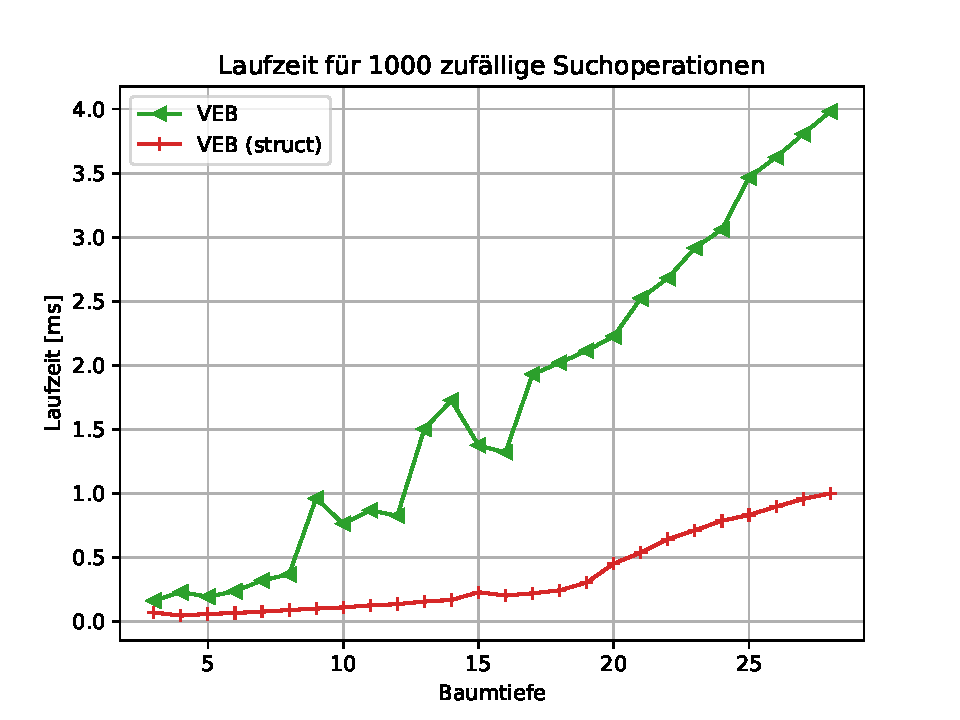
\includegraphics[scale=.6]{veb_vebstruct.pdf}
		
		
	\end{columns}
	\end{frame}
	
%------------------------------------------------

\begin{frame}
	\frametitle{Aufgabe 3.1 - Auswertung}
	\begin{columns}[c] % The "c" option specifies centered vertical alignment while the "t" option is used for top vertical alignment
		
		\column{.35\textwidth} % Left column and width
		\textbf{Vergleich der Level Implementationen}
		\begin{itemize}
			\item struct-Implementation verbraucht mindestens den \textbf{dreifachen} Speicher
		\end{itemize}
		
		\column{.6\textwidth} % Right column and width
		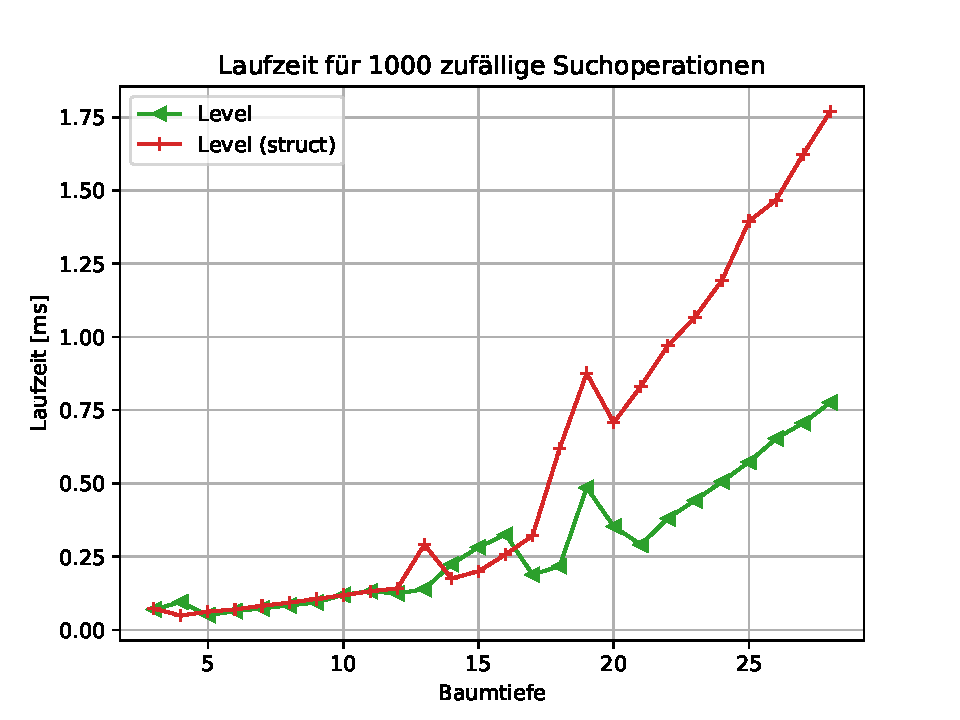
\includegraphics[scale=.6]{level_levelstruct.pdf}
		
		
	\end{columns}
	\end{frame}
	
%------------------------------------------------

\begin{frame}
	\frametitle{Aufgabe 3.1 - Auswertung}
	\begin{columns}[c] % The "c" option specifies centered vertical alignment while the "t" option is used for top vertical alignment
		
		\column{.35\textwidth} % Left column and width
		\textbf{Vergleich zur STL Implementation}
		\begin{itemize}
			\item Die struct Implementationen von VEB und Level sind schneller als \texttt{std::set}
		\end{itemize}
		
		\column{.6\textwidth} % Right column and width
		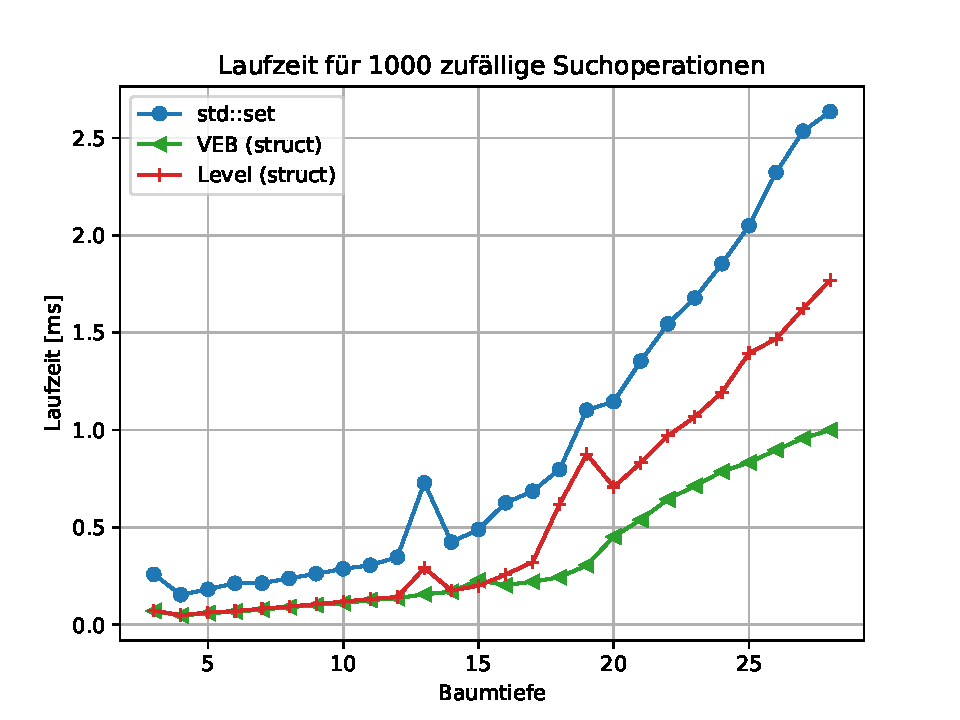
\includegraphics[scale=.6]{set_level_veb.pdf}
		
		
	\end{columns}
	\end{frame}
	
%------------------------------------------------

\begin{frame}
	\frametitle{Aufgabe 3.1 - Auswertung}
	\begin{columns}[c] % The "c" option specifies centered vertical alignment while the "t" option is used for top vertical alignment
		
		\column{.35\textwidth} % Left column and width
		Vergleich einiger Layout Implementationen und \texttt{std::set}
		
		\column{.6\textwidth} % Right column and width
		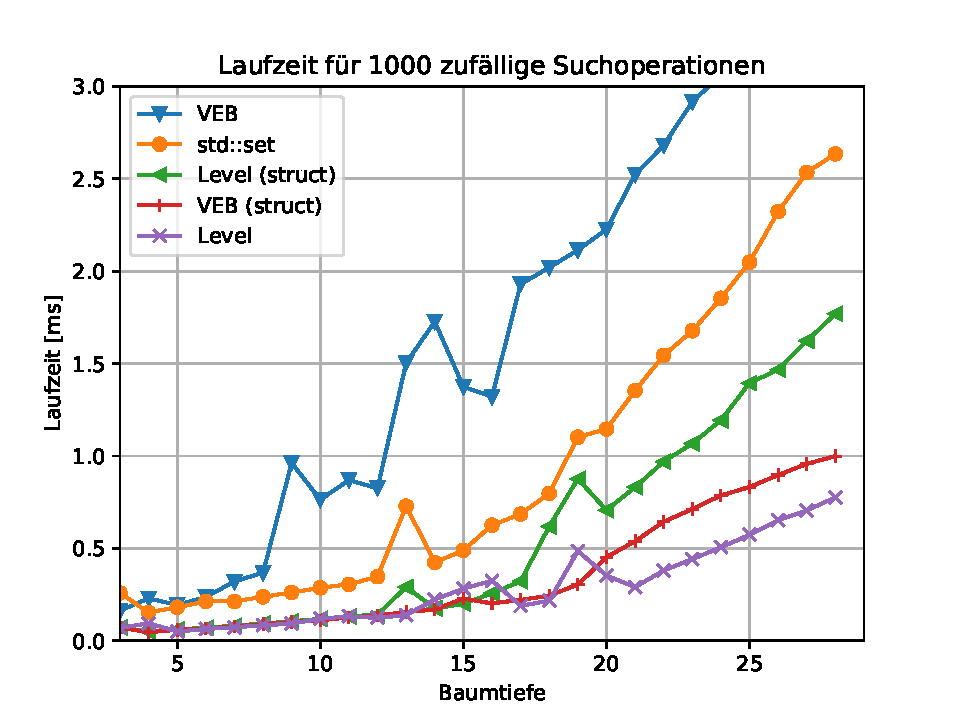
\includegraphics[scale=.6]{struct_comp.pdf}
		
		
	\end{columns}
	\end{frame}
	
%------------------------------------------------



\end{document} 